\documentclass[crop,tikz]{standalone}

\usepackage{pgfplots}
\usetikzlibrary{math}
\usetikzlibrary{calc}
\usetikzlibrary{decorations.pathreplacing, matrix}
\usetikzlibrary{pgfplots.statistics}
\pgfplotsset{compat=1.16}

\pgfplotscreateplotcyclelist{mycycle}{
black, fill=red!40,every mark/.append style={fill=blue!80!black},mark=*\\
}

\begin{document}
    

\begin{tikzpicture}
\begin{axis}[
height=4.5cm,
width=8cm,
xlabel=Number of scenarios,
ylabel=Opt number of batteries,
ylabel near ticks,
]

\foreach \i in {0,...,8}{
    \addplot[blue] table [x=w, y=\i, col sep=comma] {img/data.csv};
    \label{plot:\i};
}
%\addlegendentry{$N = 15$}
\foreach \i in {9,...,17}{
    \addplot[red] table [x=w, y=\i, col sep=comma] {img/data.csv};
    \label{plot:\i};
}
%\addlegendentry{$N = 30$}
\foreach \i in {18,...,26}{
    \addplot[black] table [x=w, y=\i, col sep=comma] {img/data.csv};
    \label{plot:\i};
}
%\addlegendentry{$N = 45$}

 \coordinate (legend) at (axis description cs:0.5,1.1);

\end{axis}
\matrix [
            draw,
            matrix of nodes,
        ] at (legend) {
            $N = 15$ \ref{plot:0} & $N=30$ \ref{plot:9}  & $N=45$ \ref{plot:18}  \\
        };
\end{tikzpicture}

\newpage

\begin{tikzpicture}
  \begin{axis}
    [
    xtick={1, ..., 8},
    xticklabels={3, ..., 10},
    ytick={0, 0.01, 0.02, 0.03, 0.04},
    boxplot/draw direction=y,
    cycle list name=mycycle,
    height=5cm,
    width=8cm,
    xlabel=Number of players,
    ylabel=$M^{S^*}(y) \slash v_d(S)$,
    ylabel near ticks,
    ]
    
\addplot+[
    boxplot prepared={
      median=0.0,
      upper quartile=0.002768822809964922,
      lower quartile=0.0,
      upper whisker=0.012797056689090027,
      lower whisker=0.0
    }
    ] coordinates {  (1, 0.02697) (1, 0.02859)  };
    
    

    \addplot+[
    boxplot prepared={
      median=0.0018507880769922267,
      upper quartile=0.004958003353515878,
      lower quartile=0.0,
      upper whisker=0.009785297092430048,
      lower whisker=0.0
    }
    ] coordinates {  (2, 0.00999)  };
    
    

    \addplot+[
    boxplot prepared={
      median=0.0,
      upper quartile=0.0015769614275916836,
      lower quartile=0.0,
      upper whisker=0.004944827040169307,
      lower whisker=0.0
    }
    ] coordinates {  (3, 0.00754) (3, 0.00779)  };
    
    

    \addplot+[
    boxplot prepared={
      median=0.0,
      upper quartile=0.000354323883027379,
      lower quartile=0.0,
      upper whisker=0.003621336282185315,
      lower whisker=0.0
    }
    ] coordinates {  (4, 0.00422)  };
    
    

    \addplot+[
    boxplot prepared={
      median=0.0,
      upper quartile=0.0007831394097133494,
      lower quartile=0.0,
      upper whisker=0.002967401506263496,
      lower whisker=0.0
    }
    ] coordinates {  (5, 0.00358)  };
    
    

    \addplot+[
    boxplot prepared={
      median=0.0,
      upper quartile=6.876887603257853e-05,
      lower quartile=0.0,
      upper whisker=0.0005555791048967684,
      lower whisker=0.0
    }
    ] coordinates {  (6, 0.00065)  };
    
    

    \addplot+[
    boxplot prepared={
      median=0.0004191070338928432,
      upper quartile=0.0005886270453638563,
      lower quartile=0.0,
      upper whisker=0.0016845010683056182,
      lower whisker=0.0
    }
    ] coordinates {  (7, 0.00219)  };
    
    

    \addplot+[
    boxplot prepared={
      median=0.0001807248858382736,
      upper quartile=0.00037228681913920996,
      lower quartile=6.703648271528544e-05,
      upper whisker=0.0007441957284442716,
      lower whisker=0.0
    }
    ] coordinates {  (8, 0.00239)  };
  \end{axis}
\end{tikzpicture}

\newpage

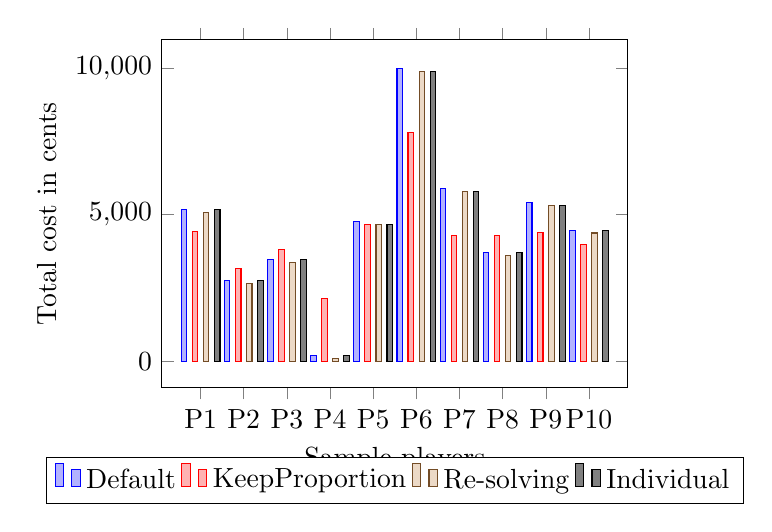
\begin{tikzpicture}
\begin{axis}[
x tick label style={
/pgf/number format/1000 sep=},
xtick={0, ..., 9},
xticklabels={P1, P2, P3, P4, P5, P6, P7, P8, P9, P10},
yticklabel style={
        /pgf/number format/fixed,
        /pgf/number format/precision=5
},
scaled y ticks=false,
%ytick={0, 1000, ..., 10000},
%yticklabels={0, 1000, ..., 10000},
ylabel=Total cost in cents,
xlabel=Sample players,
%enlargelimits=0.15,
legend style={at={(0.5,-0.20)},
anchor=north,legend columns=-1},
ybar,
bar width=2pt,
ylabel near ticks,
width=7.5cm,
height=6cm,
]
\addplot coordinates {
(0, 5164.085) (1, 2741.558) (2, 3459.796) (3, 177.717) (4, 4765.9) (5, 9975.363) (6, 5895.572) (7, 3702.434) (8, 5415.379) (9, 4463.329)
};


\addplot coordinates {
(0, 4417.117) (1, 3149.594) (2, 3821.339) (3, 2124.824) (4, 4656.924) (5, 7792.349) (6, 4279.182) (7, 4272.654) (8, 4377.481) (9, 3989.703)
};


\addplot coordinates {
(0, 5070.485) (1, 2647.958) (2, 3366.196) (3, 84.117) (4, 4672.3) (5, 9881.763) (6, 5801.972) (7, 3608.834) (8, 5321.779) (9, 4369.73)
};


\addplot coordinates {
(0, 5164.085) (1, 2741.558) (2, 3459.796) (3, 177.717) (4, 4657.9) (5, 9867.363) (6, 5787.571) (7, 3702.434) (8, 5307.379) (9, 4463.329)
};
\legend{Default, KeepProportion,Re-solving, Individual}
\end{axis}
\end{tikzpicture}


\end{document}
